\section{Report for the research project - \today}
A new family of graphs is investigated for its edge-length ratio optimization on a fixed grid. A $k$-tree is an undirected graph which is incrementally created from a $K_{k+1}$ in a way that each added vertex has exactly $k$ neighbours such that those $k+1$ vertices form a clique. Following this definition, a $4$-tree is not planar since it starts with a $K_5$. Of interest is the 2-tree and the 3-tree. 
\subsection{2-trees}
For a 2-tree, each vertex is added to exactly two neighbours, forming a clique of size 3. A 2-tree inherits two forms of structure: a parallel structure or a serial structure.
\subsubsection{Parallel case}
In the parallel case, there are parallel components between two cut vertices. The most basic component would be one vertex connected to the cut vertices, as illustrated in the following figure:
\begin{figure}[H]
	\centering
	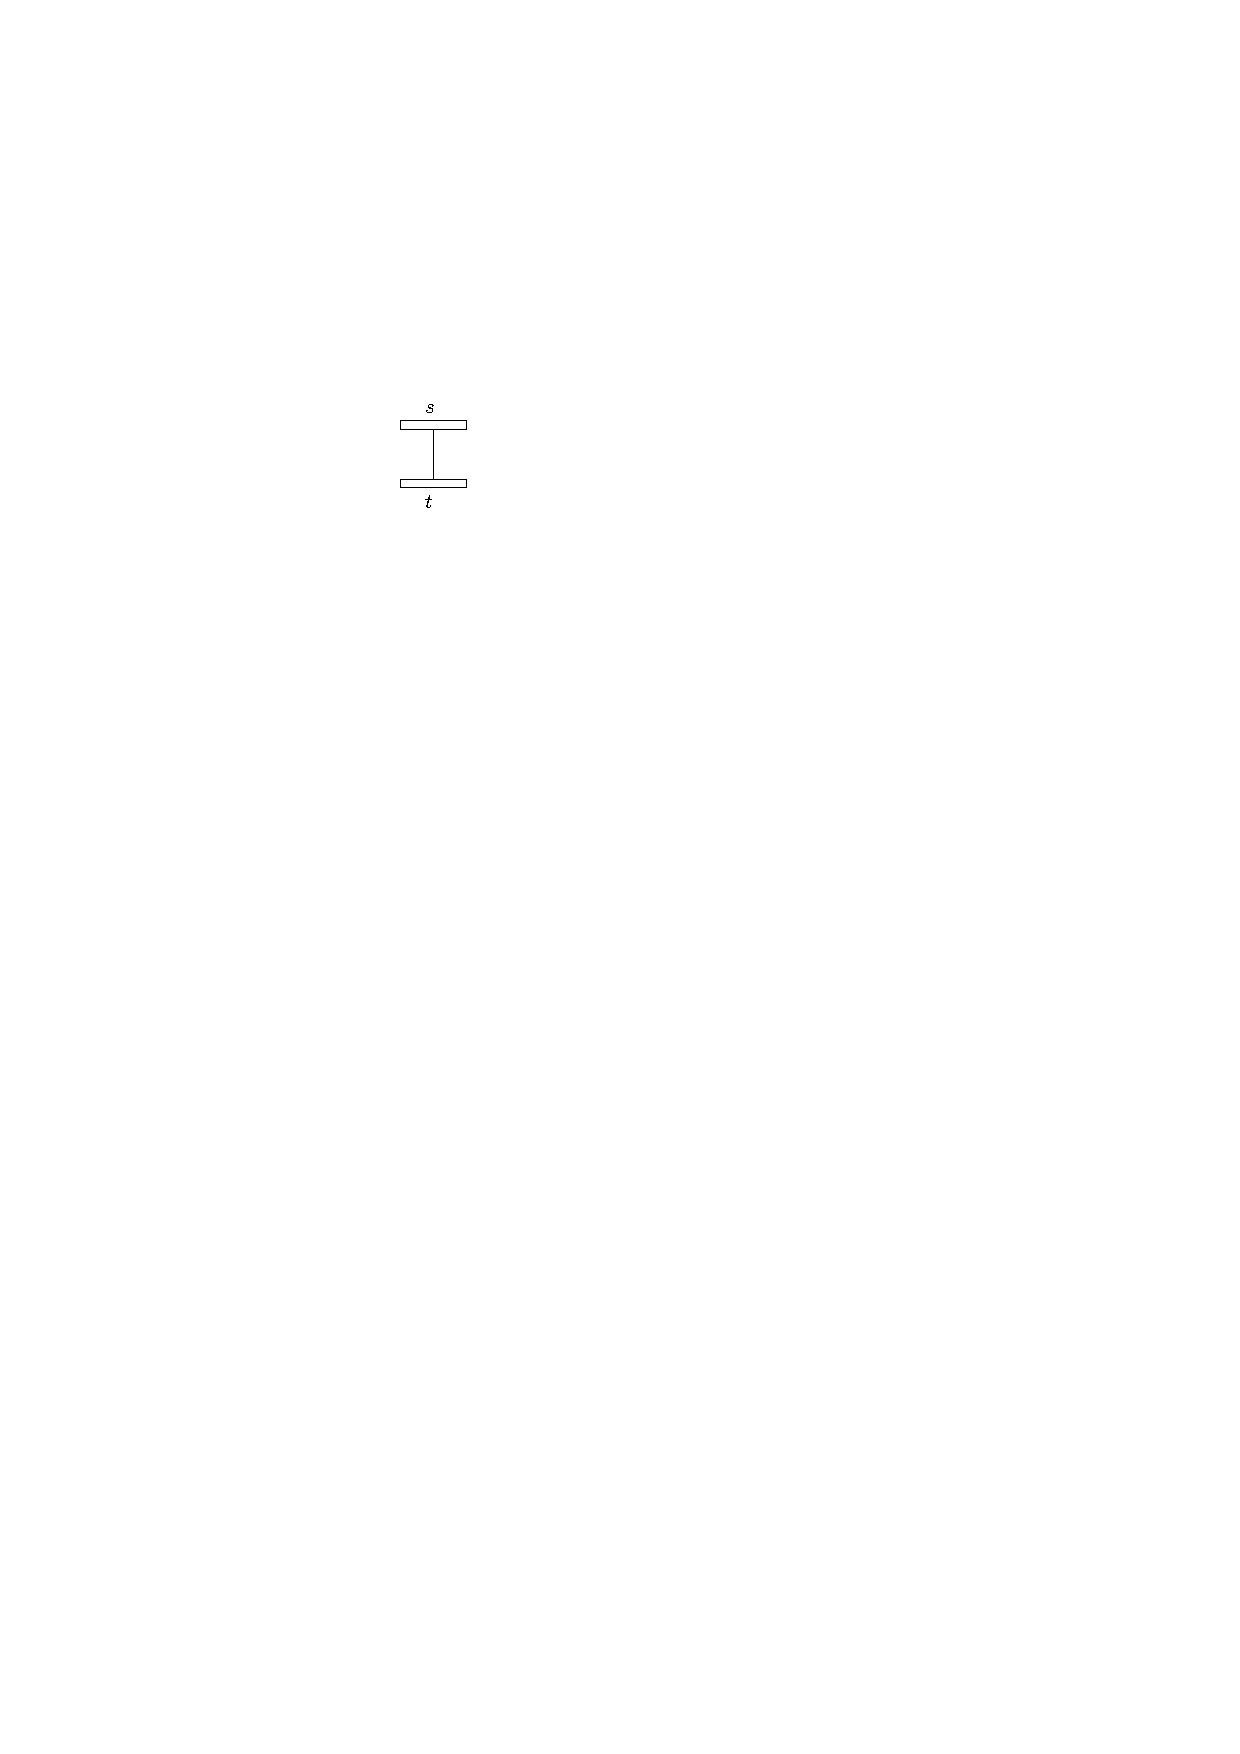
\includegraphics[width=.7\linewidth,page=1]{drawings/2-trees.pdf}
	\caption{Two cut vertices with four parallel components (for each component, there is a color), consisting of one vertex each}
\end{figure}
In the figure above, there are four parallel components. In the following, $m$ components consisting of one vertex each will be investigated.
\begin{figure}[H]
	\centering
	\includegraphics[width=.7\linewidth,page=2]{drawings/2-trees.pdf}
	\caption{Two cut vertices with $m$ parallel components}
\end{figure}
The following algorithm will draw this parallel structure with an edge-length ratio of $\mathcal{O}(1)$.\\
\begin{algorithm}[H]
	\caption{Pseudocode}
	\KwIn{Parallel structure with $m$ parallel components, consisting of one vertex each, and a constant spacing $d$}
	\KwOut{A drawing in area $2dm\times dm$, with an edge length ratio of $\mathcal{O}(1)$}
	Draw the outermost triangle with $A(0,0), B(2dm,0), C_1(dm,dm)$.\\
	\For{$i \in [2..m]$}{
		The vertex of the component $C_i(d\cdot m, d\cdot m - d\cdot (i-1))$\\
		The bend point used to connect to $A$:$K_{A_i}(1,d\cdot m - (i-1))$\\
		The bend point used to connect to $B$:$K_{B_i}(2dm-1,d\cdot m-(i-1))$
	}
\end{algorithm}
Then, for the edge $\overline{AC_m}$, the length equals:
\begin{align*}
	|\overline{AC_m}| = \sqrt{1+\left(dm-(m-1)\right)^2} + \sqrt{\left(dm-1\right)^2 + \left((d-1)(m-1)  \right)^2}
\end{align*}
\begin{lemma}
	For the spacing of $d=4$, the edge-length ratio is optimal for the above construction.
\end{lemma}
\begin{proof}
	For $d=4$, it holds:
	\begin{align}
		\lim_{m\to\infty} |\overline{AC_m}| = \sqrt{9m^2} + \sqrt{25m^2} = 8m    \label{eq:lim}
	\end{align}
	The outermost edge $\overline{AB}$ has $8m$ length. Due to the limes behaviour of the edge $AC_m$, the edge-length ratio tends to 1.
\end{proof}
\Kommentar{Ich gehe nochmal die Berechnung der Koordinaten und die Kantenlänge für $\overline{AC_m}$ durch, macht das soweit Sinn?}
The shape of the outermost triangle determines not only the edge-length ratio, but also the possibility to draw multiples of it next to each other. With the following shape, the edge-length ratio is not exactly 1 anymore, but allows us to draw consecutively.
\begin{figure}[H]
	\centering
\begin{subfigure}{0.4\textwidth}
	\centering
	\includegraphics[width=.7\linewidth,page=3]{drawings/2-trees.pdf}
	\caption{This shape reminds of a T-Shape, but has area inside so that inner parallel components could be drawn}
\end{subfigure}
\begin{subfigure}{0.4\textwidth}
	\centering
	\includegraphics[width=.7\linewidth,page=4]{drawings/2-trees.pdf}
	\caption{next to each other}
\end{subfigure}
\end{figure}
Considering the graph drawn in Figure 2, the parallel components consisting of one vertex could be connected to three vertex pairs. So, there are three cases for a drawing:
\begin{figure}[H]
	\centering
	\begin{subfigure}{0.7\textwidth}
		\centering
		\includegraphics[width=.7\linewidth,page=5]{drawings/2-trees.pdf}
		\caption{Case 1}
	\end{subfigure}
	\begin{subfigure}{0.7\textwidth}
		\centering
		\includegraphics[width=.7\linewidth,page=6]{drawings/2-trees.pdf}
		\caption{Case 2}
	\end{subfigure}
	\begin{subfigure}{0.7\textwidth}
	\centering
	\includegraphics[width=.7\linewidth,page=7]{drawings/2-trees.pdf}
	\caption{Case 3}
\end{subfigure}
\caption{Three cases of connectivity}
\end{figure}
\Kommentar{Momentan bin ich am optimieren der drei Beispiele. Ich frage mich, ob ich mit dieser Herangehensweise auf einem richtigen Weg bin. Die Parallelstrukturen könnten ja mehr sein als nur ein Knoten. Auch frage ich mich, ob ich nicht nochmal etwas vergessen habe, im Sinne von dass ich die 2-Trees immer noch nicht richtig gegriffen habe.}